\section{Considere las siguientes restricciones de un p.p.l.}
\begin{tabular}{|l|}
\hline
$x_1+x_2\leq 3 $  \\ \hline
$-2x_1+x_2\leq 2$ \\ \hline
$x_2-2x_2\leq0$   \\ \hline
$x_1, x_2 \leq 0$ \\ \hline
\end{tabular}

\begin{itemize}
    \item Grafica la región factible\\
    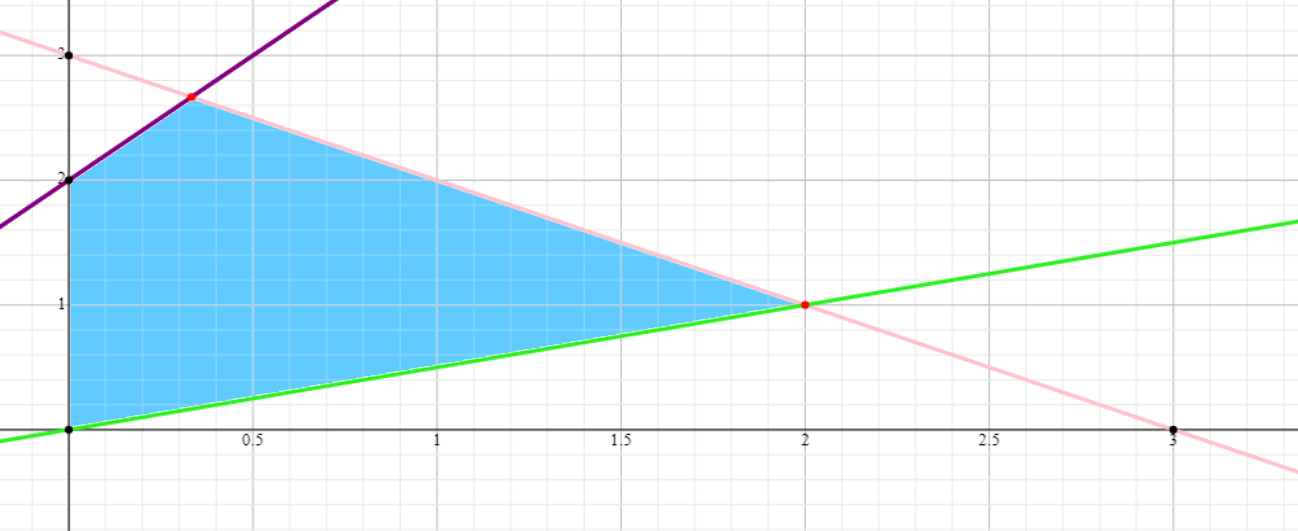
\includegraphics[scale=0.2]{Ejercicios/graficas/Ejercicio1.png}
    
    \item Identifica los puntos extremos y para cada uno de ellos identifica sus correspondientes variables básicas y no básicas.
        \begin{center}
            \begin{tabular}{|l|}
\hline
$x_1+x_2+x_3= 3 $  \\ \hline
$-2x_1+x_2+x_4= 2$ \\ \hline
$x_2-2x_2+x_5=0$   \\ \hline
$x_1, x_2 \leq 0$ \\ \hline
\end{tabular}
        \end{center}
        donde $x_i\geq 0 | i\in {1,2,3,4,5}$
        Así tenemos:
        $$A=\begin{pmatrix}1&1&1&0&0\\ -2&1&0&1&0\\ 1&-2&0&0&1\end{pmatrix}, B=\begin{pmatrix}5\\ 2\\ 0\end{pmatrix}$$
        
        Así tenemos: 
        $$\begin{pmatrix}5\\ 3\end{pmatrix}= \frac{5!}{3!\left(5-3\right)!}=10$$
        entonces:
        $$B_1=\begin{pmatrix}a_1&a_2&a_3\end{pmatrix}$$
        $$B_2=\begin{pmatrix}a_1&a_2&a_4\end{pmatrix}$$
        $$B_3=\begin{pmatrix}a_1&a_2&a_5\end{pmatrix}$$
        $$B_4=\begin{pmatrix}a_1&a_3&a_4\end{pmatrix}$$
        $$B_5=\begin{pmatrix}a_1&a_3&a_5\end{pmatrix}$$
        $$B_6=\begin{pmatrix}a_1&a_4&a_5\end{pmatrix}$$
        $$B_7=\begin{pmatrix}a_2&a_3&a_4\end{pmatrix}$$
        $$B_8=\begin{pmatrix}a_2&a_3&a_5\end{pmatrix}$$
        $$B_9=\begin{pmatrix}a_2&a_4&a_5\end{pmatrix}$$
        $$B_{10}=\begin{pmatrix}a_3&a_4&a_5\end{pmatrix}$$
        
    Así tenemos que:
    $$B_1=\begin{pmatrix}1&1&1\\ -2&1&0\\ 1&-2&0\end{pmatrix}\Rightarrow B_1^{-1}=\begin{pmatrix}0&-\frac{2}{3}&-\frac{1}{3}\\ 0&-\frac{1}{3}&-\frac{2}{3}\\ 1&1&1\end{pmatrix}, X_{B_1}=\begin{pmatrix}x_1\\ x_2\\ x_3\end{pmatrix}$$
    $$\rightarrow X_{B_{1}}=B_1^{-1}b=\begin{pmatrix}1&1&1\\ -2&1&0\\ 1&-2&0\end{pmatrix}\begin{pmatrix}3\\ 2\\ 0\end{pmatrix}=\begin{pmatrix}-\frac{4}{3}\\ -\frac{2}{3}\\ 5\end{pmatrix}\begin{pmatrix}x_1\\ x_2\\ x_3\end{pmatrix}$$
    $\therefore X_{B_{1}}^{t}=\begin{pmatrix}-\frac{4}{3}&-\frac{2}{3}&5&0&0\end{pmatrix}$ \textsc{Variable básica no factible}
    
    $$B_2=\begin{pmatrix}1&1&0\\ -2&1&1\\ 1&-2&0\end{pmatrix}\Rightarrow B_2^{-1}=\begin{pmatrix}\frac{2}{3}&0&\frac{1}{3}\\ \frac{1}{3}&0&-\frac{1}{3}\\ 1&1&1\end{pmatrix}, X_{B_2}=\begin{pmatrix}x_1\\ x_2\\ x_4\end{pmatrix}$$
    $$\rightarrow X_{B_2}=B_2^{-1}b\begin{pmatrix}\frac{2}{3}&0&\frac{1}{3}\\ \frac{1}{3}&0&-\frac{1}{3}\\ 1&1&1\end{pmatrix}\begin{pmatrix}3\\ 2\\ 0\end{pmatrix}=\begin{pmatrix}2\\ 1\\ 5\end{pmatrix}\begin{pmatrix}x_1\\ x_2\\ x_4\end{pmatrix}$$
    $\therefore X_{B_2}^t=\begin{pmatrix}\frac{1}{3}&\frac{8}{3}&0&0&5\end{pmatrix}$ \textsc{Variable básica factible}
    $$B_3=\begin{pmatrix}1&1&0\\ -2&1&0\\ 1&-2&1\end{pmatrix}\Rightarrow B_3^{-1}=\begin{pmatrix}\frac{1}{3}&-\frac{1}{3}&0\\ \frac{2}{3}&\frac{1}{3}&0\\ 1&1&1\end{pmatrix}, X_{B_3}=\begin{pmatrix}x_1\\ x_2\\ x_5\end{pmatrix}$$
    $$\rightarrow \:X_{B_3}=B_3^{-1}b=\begin{pmatrix}\frac{1}{3}&-\frac{1}{3}&0\\ \frac{2}{3}&\frac{1}{3}&0\\ 1&1&1\end{pmatrix}\begin{pmatrix}3\\ 2\\ 1\end{pmatrix}=\begin{pmatrix}\frac{1}{3}\\ \frac{8}{3}\\ 5\end{pmatrix}\begin{pmatrix}x_1\\ x_2\\ x_5\end{pmatrix}$$
    $\therefore X_{B_3}^t=\begin{pmatrix}\frac{1}{3}&\frac{8}{3}&0&0&5\end{pmatrix}$ \textsc{Variable  básica factible}
    $$B_4=\begin{pmatrix}1&1&0\\ -2&0&1\\ 1&0&0\end{pmatrix}\Rightarrow B_4^{-1}=\begin{pmatrix}0&0&1\\ 1&0&-1\\ 0&1&2\end{pmatrix}, X_{B_4}=\begin{pmatrix}x_1\\ x_3\\ x_4\end{pmatrix}$$
    $$\rightarrow X_{B_4}=B_4^{-1}b=\begin{pmatrix}0&0&1\\ 1&0&-1\\ 0&1&2\end{pmatrix}\begin{pmatrix}3\\ 2\\ 0\end{pmatrix}=\begin{pmatrix}0\\ 3\\ 2\end{pmatrix}\begin{pmatrix}x_1\\ x_3\\ x_4\end{pmatrix}$$
    $\therefore X_{B_4}^t=\begin{pmatrix}0&0&3&2&0\end{pmatrix}$ \textsc{Variable  básica factible}
    $$ B_5=\begin{pmatrix}1&1&0\\ -2&0&0\\ 1&0&1\end{pmatrix}\Rightarrow B_5^{-1}=\begin{pmatrix}0&\frac{1}{2}&0\\ 1&\frac{1}{2}&0\\ 0&\frac{1}{2}&1\end{pmatrix},\:X_{B_5}=\begin{pmatrix}x_1\\ x_3\\ x_5\end{pmatrix} $$
    $$\rightarrow \:X_{B_5}=B_5^{-1}b=\begin{pmatrix}0&\frac{1}{2}&0\\ \:1&\frac{1}{2}&0\\ \:0&\frac{1}{2}&1\end{pmatrix}\begin{pmatrix}3\\ \:2\\ \:0\end{pmatrix}=\begin{pmatrix}-1\\ \:4\\ \:1\end{pmatrix}\begin{pmatrix}x_1\\ \:x_3\\ \:x_5\end{pmatrix}$$
    $\therefore X_{B_5}^t=\begin{pmatrix}-1&0&4&0&1\end{pmatrix}$ \textsc{Variable  básica no factible}
    
    $$B_6=\begin{pmatrix}1&0&0\\ -2&1&0\\ 1&0&2\end{pmatrix}\Rightarrow B_6^{-1}=\begin{pmatrix}1&0&0\\ 2&1&0\\ -1&0&1\end{pmatrix},\:X_{B_6}=\begin{pmatrix}x_1\\ x_4\\ x_5\end{pmatrix}$$
    $$\rightarrow X_{B_6}=B_6^{-1}b=\begin{pmatrix}1&0&0\\ 2&1&0\\ -1&0&1\end{pmatrix}\begin{pmatrix}3\\ 2\\ 0\end{pmatrix}=\begin{pmatrix}3\\ 8\\ -1\end{pmatrix}\begin{pmatrix}x_1\\ x_4\\ x_5\end{pmatrix}$$   
    $\therefore X_{B_6}^t=\begin{pmatrix}3&0&0&8&-3\end{pmatrix}$ \textsc{Variable  básica no factible}
    
    $$B_7=\begin{pmatrix}1&1&0\\ 1&0&1\\ -2&0&0\end{pmatrix}\Rightarrow \:B_7^{-1}=\begin{pmatrix}0&0&\frac{1}{2}\\ 1&0&\frac{1}{2}\\ 0&1&\frac{1}{2}\end{pmatrix},\:X_{B_7}=\begin{pmatrix}x_2\\ x_3\\ x_4\end{pmatrix}$$
    $$\rightarrow \:X_{B_7}=B_7^{-1}b=\begin{pmatrix}1&1&0\\ 1&0&1\\ -2&0&0\end{pmatrix}\Rightarrow \:B_7^{-1}=\begin{pmatrix}0&0&-\frac{1}{2}\\ 1&0&\frac{1}{2}\\ 0&1&\frac{1}{2}\end{pmatrix},\:X_{B_7}=\begin{pmatrix}x_2\\ x_3\\ x_4\end{pmatrix}$$
    $\therefore X_{B_7}^t=\begin{pmatrix}0&0&3&2&0\end{pmatrix}$ \textsc{Variable  básica factible}
    
    $$B_8=\begin{pmatrix}1&1&0\\ 1&0&0\\ -2&0&1\end{pmatrix}\Rightarrow \:B_8^{-1}=\begin{pmatrix}0&1&0\\ 1&-1&0\\ 0&2&1\end{pmatrix},\:X_{B_8}=\begin{pmatrix}x_2\\ x_3\\ x_5\end{pmatrix}$$
    
    $$\rightarrow \:X_{B_8}=B_8^{-1}b=\begin{pmatrix}0&1&0\\ 1&-1&0\\ 0&2&1\end{pmatrix}\begin{pmatrix}3\\ 2\\ 0\end{pmatrix}=\begin{pmatrix}2\\ 1\\ 4\end{pmatrix}\begin{pmatrix}x_2\\ x_3\\ x_5\end{pmatrix}$$
    $\therefore X_{B_8}^t=\begin{pmatrix}0&2&1&0&4\end{pmatrix}$ \textsc{Variable  básica factible}
    
    $$B_9=\begin{pmatrix}1&0&0\\ 1&1&0\\ -2&0&1\end{pmatrix}\Rightarrow \:B_9^{-1}=\begin{pmatrix}1&0&0\\ -1&1&0\\ 2&0&1\end{pmatrix},\:X_{B_9}=\begin{pmatrix}x_2\\ x_4\\ x_5\end{pmatrix}$$
    $$\rightarrow \:X_{B_9}=B_9^{-1}b=\begin{pmatrix}1&0&0\\ -1&2&0\\ 2&0&1\end{pmatrix}\begin{pmatrix}3\\ 2\\ 0\end{pmatrix}=\begin{pmatrix}3\\ -1\\ 6\end{pmatrix}\begin{pmatrix}x_2\\ x_4\\ x_5\end{pmatrix}$$
    $\therefore X_{B_9}^t=\begin{pmatrix}0&3&0&-1&6\end{pmatrix}$ \textsc{Variable  básica no factible}
    $$B_{10}=B_{10}^{-1}\begin{pmatrix}1&0&0\\ 0&1&0\\ 0&0&1\end{pmatrix},\:X_{B_{10}}=\begin{pmatrix}x_3\\ x_4\\ x_5\end{pmatrix}$$
    $$X_{B_{10}}=B_{10}^{-1}b=\begin{pmatrix}1&0&0\\ 0&1&0\\ 0&0&1\end{pmatrix}\begin{pmatrix}3\\ 2\\ 0\end{pmatrix}=\begin{pmatrix}3\\ \:2\\ \:0\end{pmatrix}\begin{pmatrix}x_3\\ x_4\\ x_5\end{pmatrix}$$
    $\therefore X_{B_{10}}^t=\begin{pmatrix}0&0&3&2&0\end{pmatrix}$  \textsc{Variable  básica factible}
    
    
    \item Suponga que se realiza un movimiento del punto extremo (2,1) al punto extremo (0, 0) en el espacio $(x_1, x_2)$ Especifica cual es la variable entrante y la saliente
    
    Tenemos que la variable entrante es $\begin{pmatrix}0&0&3&2&0\end{pmatrix}$ por lo tanto:
    $\text{Min}\:x_0=x_3+x_4+x_5$\\
    
    
    \begin{tabular}{|l|l|l|l|l|l|l|}
\hline
x_0 & x_1 & x_2 & x_3 & x_4 & x_5 & R++S \\ \hline
1   & 0   & 0   & -1  & -1  & -1  & 0    \\ \hline
0   & 1   & 1   & 1   & 0   & 0   & 3    \\ \hline
0   & -2  & 1   & 0   & 1   & 0   & 2    \\ \hline
0   & 1   & -2  & 0   & 0   & 1   & 0    \\ \hline
\end{tabular}
$\Rightarrow$
\begin{tabular}{|l|l|l|l|l|l|l|}
\hline
x_0 & x_1 & x_2 & x_3 & x_4 & x_5 & R++S \\ \hline
1   & 0   & 0   & 0   & 0   & 0   & 5    \\ \hline
0   & 1   & 1   & 1   & 0   & 0   & 3    \\ \hline
0   & -2  & 1   & 0   & 1   & 0   & 2    \\ \hline
0   & 1   & -2  & 0   & 0   & 1   & 0    \\ \hline
\end{tabular}
\end{itemize}

$\therefore$ \textsc{La solución es óptima}